\section{ETL · Construcción de la tabla maestra}

\begin{takeaway}
Siete tablas de origen, casi 1.5\,GB de datos crudos, se transforman en \textbf{una única tabla semanal nacional} con 258 filas (semanas) y las variables que alimentan el modelo. Todo parte de aquí: si la tabla está mal, el modelo está mal.
\end{takeaway}

\subsection{Contexto}

El caso nos entrega siete archivos CSV en la carpeta \texttt{data/lake/}. Los más pesados son \texttt{pedidos.csv} ($\sim$540\,MB) y \texttt{ventas\_lineas.csv} ($\sim$965\,MB) — millones de filas a nivel línea de pedido. El modelo, en cambio, necesita \textbf{semanas}, no líneas. El trabajo del ETL es agregar, limpiar y unir.

\subsection{Decisiones clave}

\begin{decisionbox}
\textbf{Granularidad:} \textit{semanal nacional}. Todas las fechas se normalizan al lunes ISO de su semana, y las diez ciudades se suman. Se pierde detalle geográfico, pero se gana una serie temporal limpia de 258 semanas alineadas con el gasto publicitario.
\end{decisionbox}

\begin{decisionbox}
\textbf{Target ($Y_t$):} \texttt{venta\_neta\_total\_eur}, la suma semanal de \texttt{venta\_neta\_sin\_iva\_eur} de \texttt{ventas\_lineas}. Es la variable que el modelo intentará explicar.
\end{decisionbox}

\begin{decisionbox}
\textbf{Ticket medio:} se calcula desde \texttt{pedidos.csv}, no desde líneas. Calcularlo sobre líneas infla el ticket, porque cada pedido tiene varias líneas pero un solo cliente y un solo carrito.
\end{decisionbox}

\begin{decisionbox}
\textbf{Tráfico excluido del modelo:} las métricas de \texttt{trafico\_tienda\_web\_diario.csv} (visitas web, tráfico tienda) son \textit{mediadores}: están \textit{después} de la inversión publicitaria en la cadena causal. Incluirlas robaría protagonismo a los canales de marketing y haría creer que el tráfico por sí solo vende. Se usan únicamente para exploración.
\end{decisionbox}

\subsection{Flujo del ETL}

\begin{enumerate}[leftmargin=*, itemsep=1pt]
    \item \textbf{Carga} de los siete CSV.
    \item \textbf{Normalización de fechas} al lunes ISO.
    \item \textbf{Agregación semanal nacional} para cada tabla.
    \item \textbf{Pivote de la inversión} por \texttt{canal\_medio} $\rightarrow$ 8 columnas \texttt{inv\_*}.
    \item \textbf{Merge LEFT desde ventas}: la tabla de ventas actúa como esqueleto; las demás se unen preservando todas las semanas con actividad comercial.
    \item \textbf{Filtrado temporal} al rango \textit{2020-01-06} $\rightarrow$ \textit{2024-12-14}, desde la primera semana con inversión registrada.
\end{enumerate}

\subsection{Validación visual}

\begin{figure}[htbp]
\centering
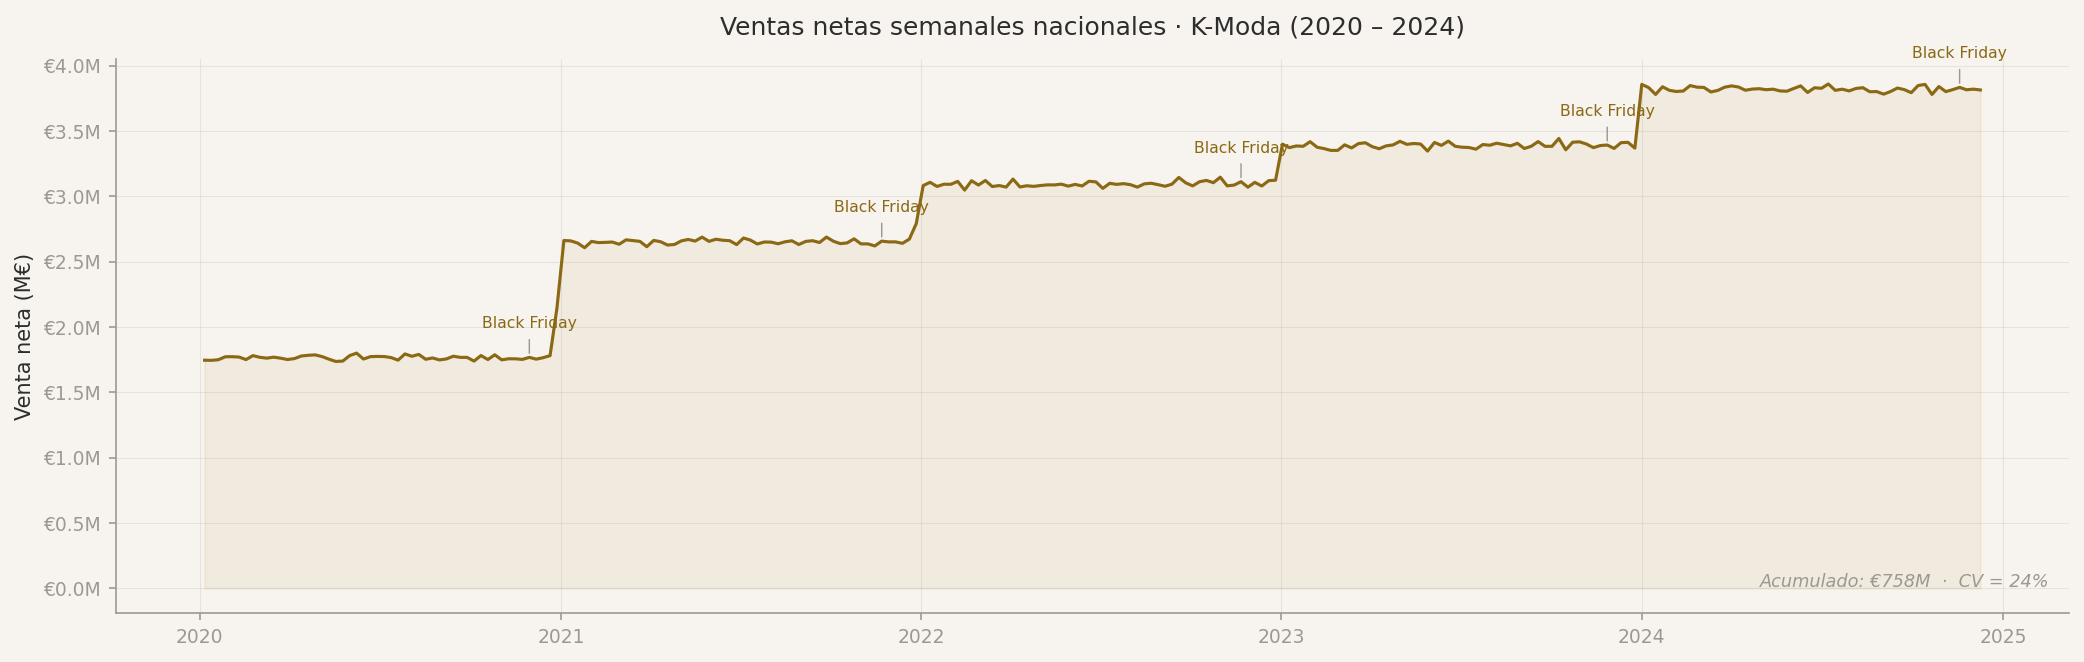
\includegraphics[width=\textwidth]{figures/g1_ventas_semanales.png}
\caption{\textbf{Ventas netas semanales 2020--2024.} El target del modelo. Se observan claramente los picos de Black Friday y los escalones anuales que reflejan el crecimiento estructural del negocio.}
\label{fig:ventas_semanales}
\end{figure}

\begin{figure}[htbp]
\centering
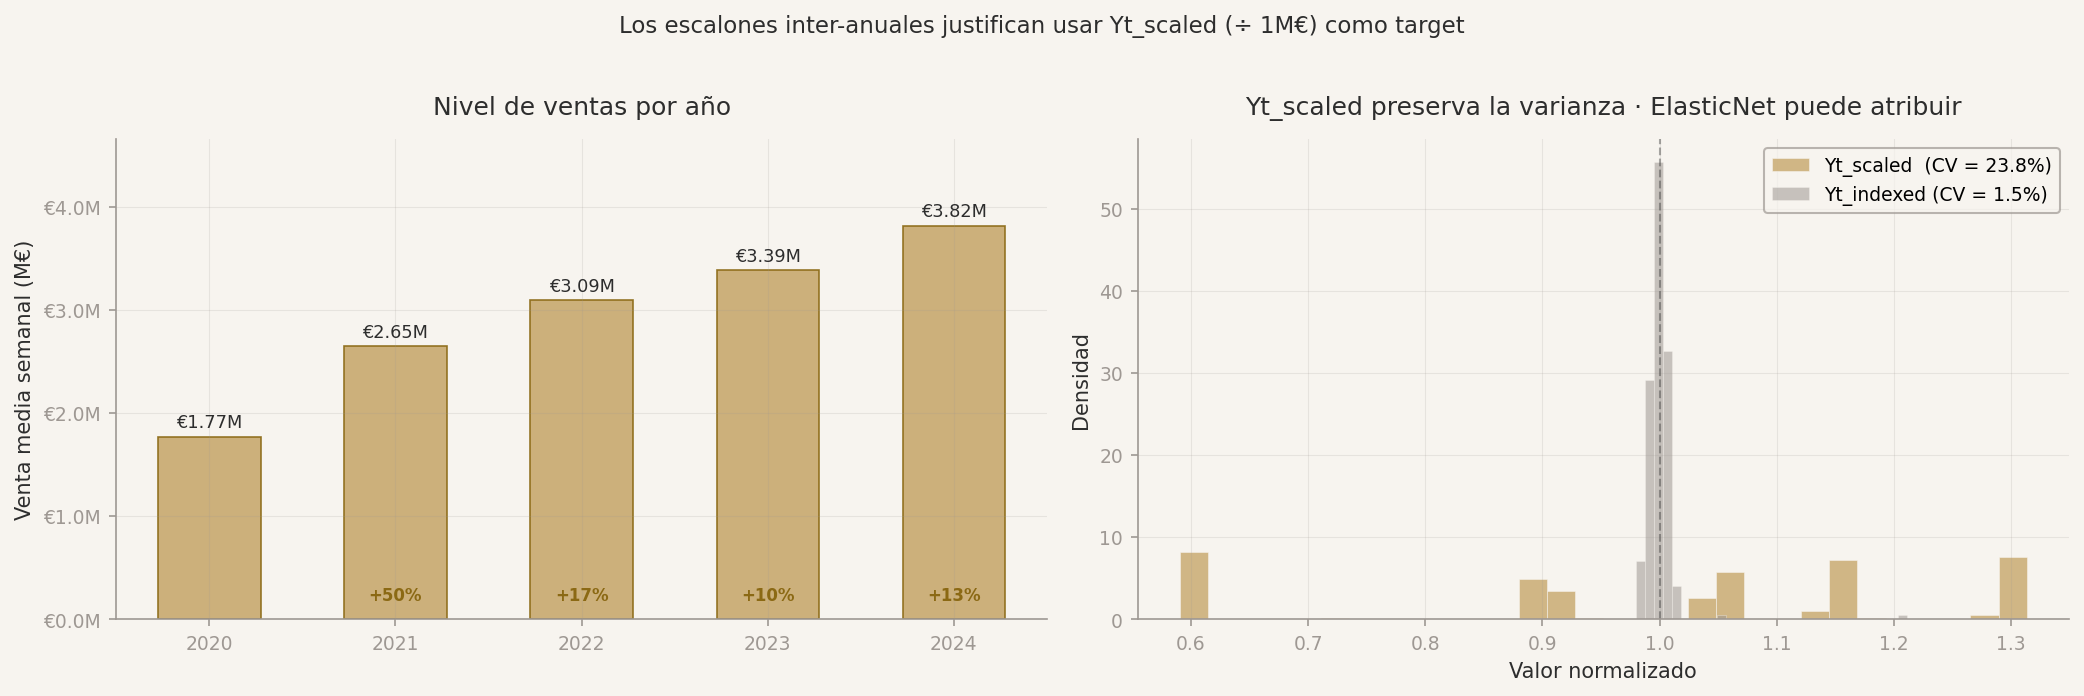
\includegraphics[width=\textwidth]{figures/g2_escalones_y_cv.png}
\caption{\textbf{Escalones anuales del target.} El nivel medio anual sube de forma discreta cada enero ($+30$--$50\%$ entre 2020 y 2021). Esta propiedad motiva las decisiones posteriores de target y de \textit{split} train/test.}
\label{fig:escalones}
\end{figure}

\begin{figure}[htbp]
\centering
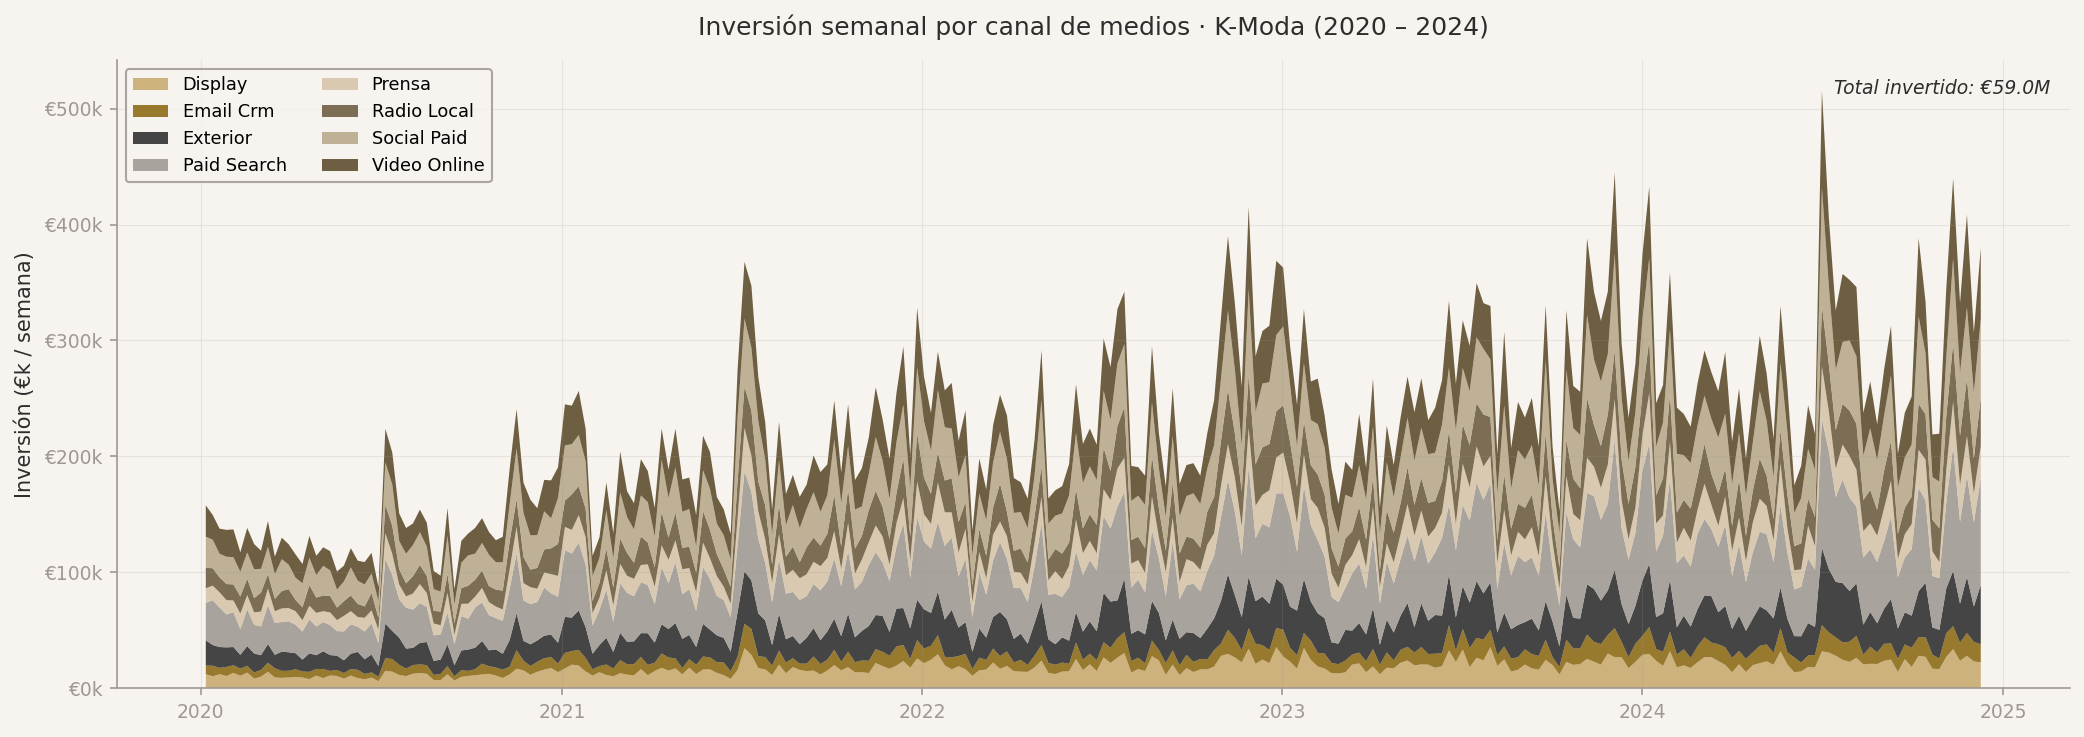
\includegraphics[width=\textwidth]{figures/g3_inversion_canales.png}
\caption{\textbf{Inversión semanal apilada por canal.} Muestra qué canales absorben más presupuesto y si hay estacionalidad o discontinuidades en el gasto.}
\label{fig:inversion}
\end{figure}

\begin{figure}[htbp]
\centering
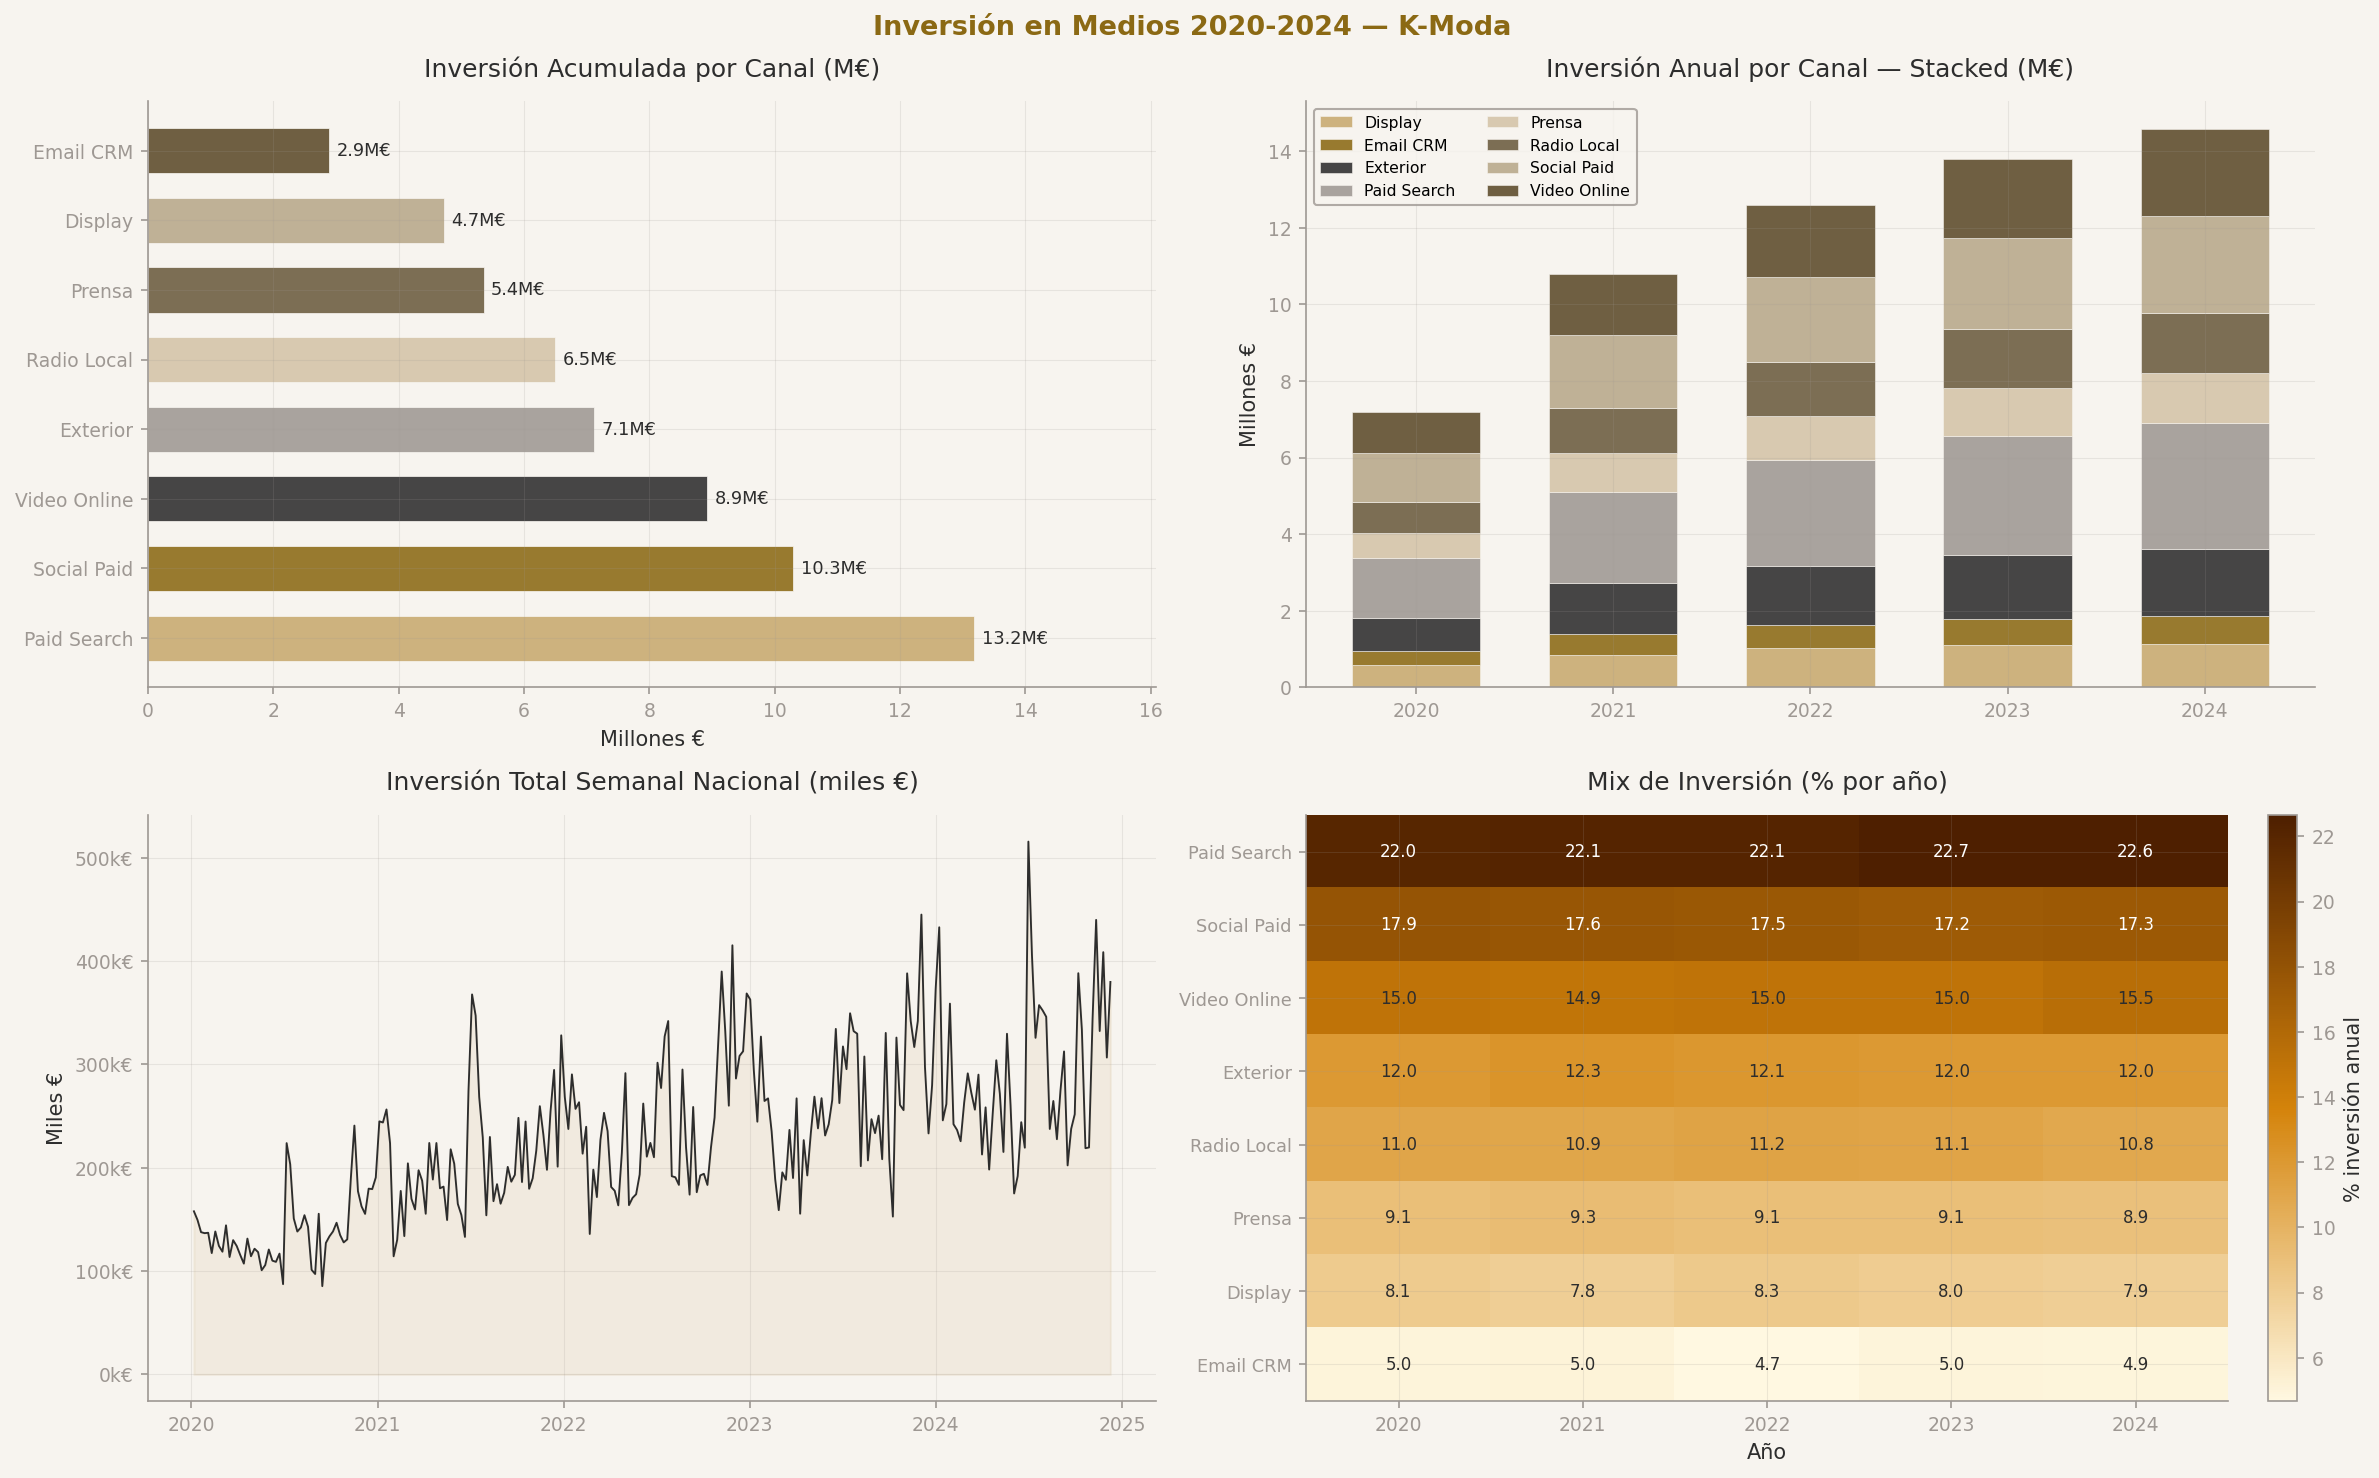
\includegraphics[width=\textwidth]{figures/inversion_medios_overview.png}
\caption{\textbf{Overview completo de la inversión en medios}: distribución por canal, evolución, composición. Vista 360º del presupuesto antes de agrupar.}
\label{fig:inv_overview}
\end{figure}

\begin{figure}[htbp]
\centering
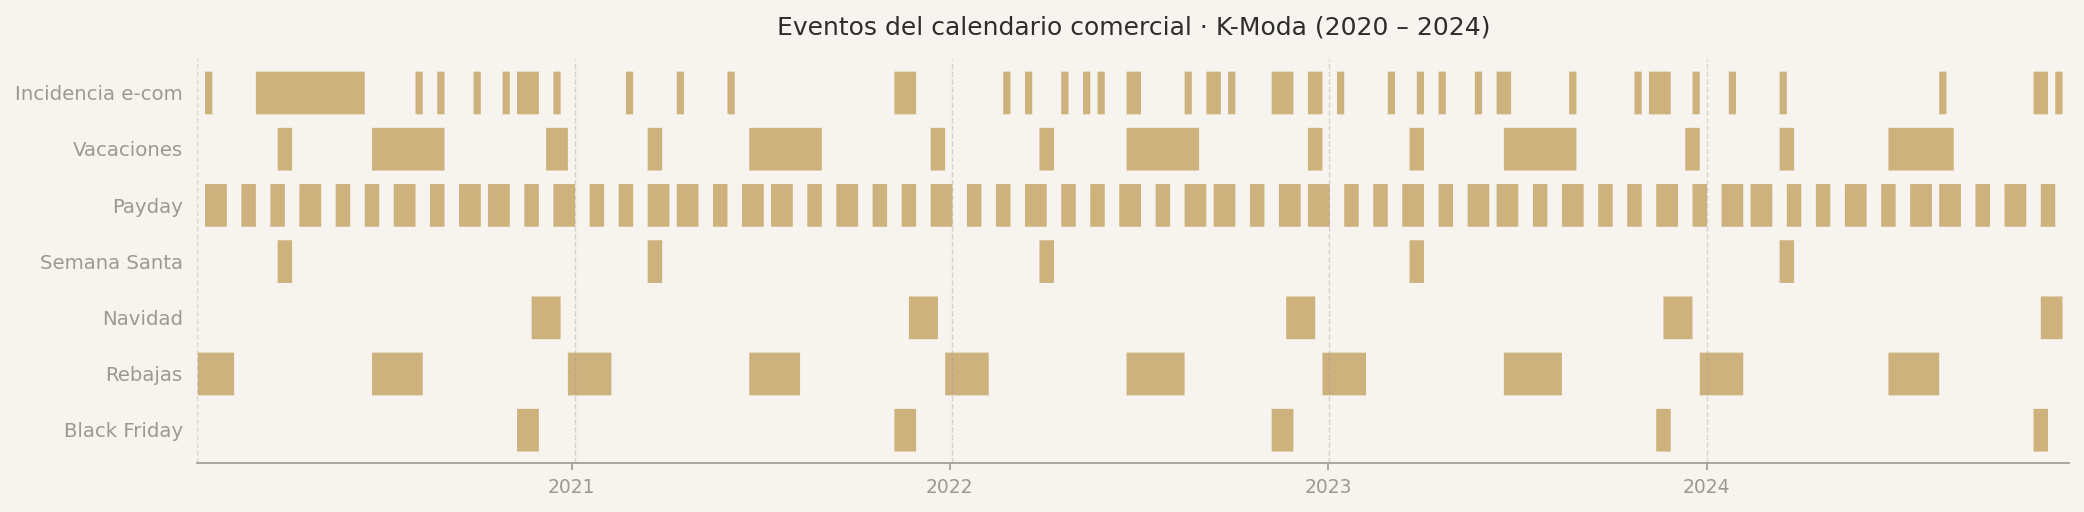
\includegraphics[width=\textwidth]{figures/g4_calendario.png}
\caption{\textbf{Calendario comercial.} Presencia semanal de los siete eventos nacionales (\textit{Black Friday}, rebajas, Navidad, etc.). Son covariables clave porque coinciden con los picos de venta y el modelo debe separarlos del efecto del marketing.}
\label{fig:calendario}
\end{figure}

\begin{figure}[htbp]
\centering
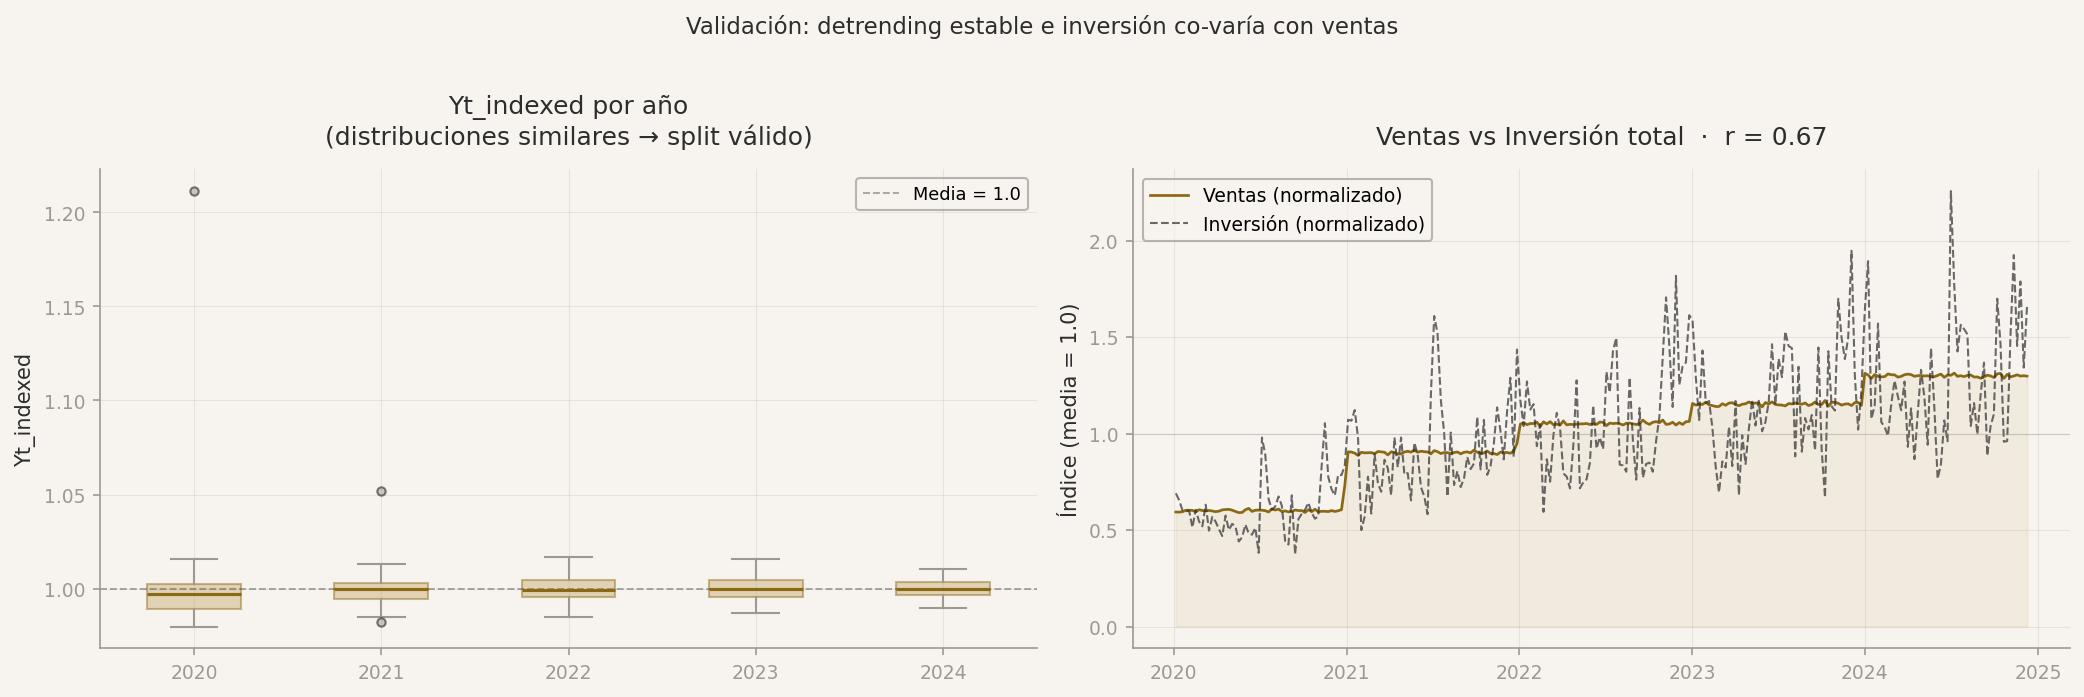
\includegraphics[width=0.95\textwidth]{figures/g5_validacion.png}
\caption{\textbf{Validación del target.} Distribuciones por año e inversión semanal total, utilizadas como sanity check antes de pasar a la fase de modelado.}
\label{fig:validacion_etl}
\end{figure}

\subsection{Resultado}

La salida del ETL es un único fichero (\texttt{etl.csv}) con 258 filas semanales y las columnas necesarias para el resto del pipeline: \texttt{semana\_inicio}, \texttt{venta\_neta\_total\_eur} (target), ocho columnas \texttt{inv\_*} (canales de inversión) y las variables de calendario y clima que actuarán como controles.
